\documentclass{IEEEtran}

\usepackage{graphicx} % Required for inserting images

\usepackage[backend=biber]{biblatex}
\addbibresource{refs.bib}

\title{Information Retrieval Project Proposal \\ Domain Adaptation using Parameter Efficient Fine Tuning (PEFT)}
\author{Janneke Nouwen (s1101750), Daan Brugmans (s1080742), Julian Roddeman (s1080491)}
\date{\today}

\begin{document}

\maketitle

\section{Introduction}
According to this study \cite{thakur2021beir}, sparse and dense LLM-based retrieval models like BERT (Bidirectional Encoder Representations) are less capable of making predictions in unseen domains. BERT is a complex model, fine-tuning all 110 million trainable parameters of the model for an unseen domain is highly expensive, and the overcomplexity of fine-tuning on this number of parameters can lead to overfitting \cite{bejani2021systematic}. \\
Parameter Efficient Fine Tuning (PEFT) approaches only fine-tune a small, new set of parameters while keeping the original parameters of the models frozen. This enables rapid adaptations of pre-trained language models to varied domains without fine-tuning the original parameters of the model, lowering computational and storage costs significantly. Because only a small number of parameters is used, this method of fine-tuning is less susceptible to overfitting \cite{Soekhoe2016}.
In this research we will compare the capability of plain BERT to classify unseen documents to a fine-tuned approach using Parameter Efficient Fine Tuning (PEFT) on BERT. \\
We will use the TREC-COVID dataset from the BEIR framework \cite{thakur2021beir, voorhees2021trec} to determine the model's capability to classify documents in an unseen domain. This decision is based on the fact that BERT was pre-trained solely on an unlabeled, plain text corpus \cite{devlin2018bert} and has no exposure to literature pertaining to the COVID-19 virus, given that its training data predates the pandemic. As a result, the specificity and freshness of the COVID-19 topic certainly designates it as an unseen domain for the model, establishing a valid dataset to assess PEFTs potential to boost the performance of classifying documents of an unseen domain.

\section{Research Question}
How can a Parameter Efficient Fine Tuning (PEFT) method improve the performance of BERT for classifying documents in unseen domains, when we compare it to a plain BERT setup?

\section{Resources}
Python 3.10 will be used to test plain BERT and BERT fine-tuned with PEFT. To apply different PEFT methods to BERT, the 'adapter-hub' library will be used \cite{pfeiffer2020}. We will compare the results using the Scikit-learn package's precision, F1-score and recall \cite{scikit-learn}. For data preprocessing, Numpy and Pandas will be used \cite{harris2020array, mckinney2010data}. 

\section{Experimental Design}

\textbf{Objective:} Our objective is to compare the capability of BERT to classify documents in an unseen domain, comparing a non-fine-tuned plain version of BERT with a dense layer, against a fine-tuned approach with PEFT. We will do this in an unseen domain, specifically in a Covid-19 domain. In figure 1, a flowchart shows the experimental setup.
\textbf{Hypothesis:} We expect that PEFT will enable BERT to effectively classify documents in an unseen (COVID-19) domain with improved performance compared to a plain BERT model. 
\textbf{Independent Variable:} Fine-tuning approach (plain BERT vs. fine-tuned BERT using PEFT)
\textbf{Dependent Variable:} Model’s performance in classifying relevancy labels of COVID-19 documents using the precision, recall and F1-score.

\begin{figure}[h]
    \centering
    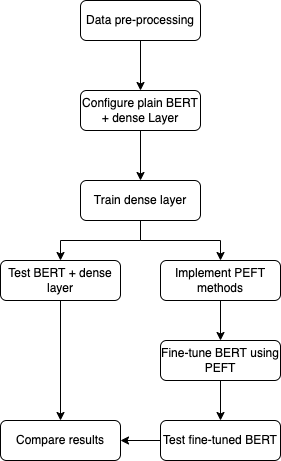
\includegraphics[width=0.30\textwidth]{flowchart.drawio.png}
    \caption{Flowchart of the experiment setup}
    \label{fig:my_image}
\end{figure}

\printbibliography

\end{document}
